\section{Radix Sort}
\label{sec:radix sort}

This section presents a parallelised algorithm of the radix sort benchmarked with a serial sort implementation from the \verb!C++! library.
The implementation of the Radix Sort algorithm can be found in \cref{ap:radix sort}.
Radix Sort is a bit-wise comparison algorithm that iteratively, in the length of the bits of the integer, looks at the least significant bit (LSB) and sorts the values accordingly.~\cite{udacity}

In order to parallelise the sorting of the LSB in the radix sort we used the compact(\cref{sec:compact}).  
Thus to parallelise the entire sorting we perform multiple compact operations as we move the elements in the array according to their LSB.
In this section we outline a single iteration of radix sort in this section.

To sort the elements according to their LSB we perform two compact operations.
The first compact operation maps the elements with LSB = 0 from the output array's zero index and up to 
\[\mathtt{zeros\_end\_idx} = \{|x|-1\ \bigg|\ (x\&1)=0, x \in \mathrm{input}\},\]
as illustrated in \cref{fig:radix sort example}.
The second compact operation maps the elements with LSB = $1$ from the output arraysindex $\mathtt{zeros\_end\_idx}+1$ to index \[\{|x|-1\}\] being the end position.  

For each iteration of Radix Sort the LSB will shift left and compact sorting thus based on increasing importance of the bit representations in the element.
Consider for instance the following
\[\mathrm{iteration 0:}0000 0000 0000 000[0]\]
\[\mathrm{iteration 1:}0000 0000 0000 00[0]0\]
\[ \ldots \]
\[\mathrm{iteration 31:}[0]000 0000 0000 0000\]

\begin{figure}[htb]
  \centering
  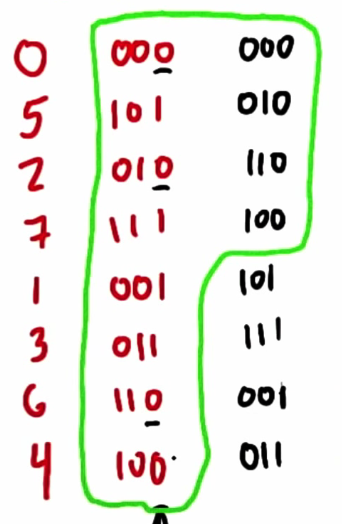
\includegraphics[height=4cm]{images/radix-sort-example.png}
  \caption{Example of how each digit is moved according to LSB}
  \label{fig:radix sort example}
\end{figure}


%\subsection*{Iterating through each Bit}
%
%\begin{lstlisting}
%for ( unsigned int i = 0; i < (BITS_PER_BYTE * sizeof( unsigned int)); i++) {
%  // predicate is that LSB is 0
%  predicate_kernel<<<GRID_SIZE, BLOCK_SIZE>>>(d_predicate, d_val_src, NUM_ELEMS, i);
%  // calculate scatter addresses from predicates
%  exclusive_sum_scan(d_sum_scan_0, d_predicate, d_predicate_tmp, d_sum_scan, ARRAY_BYTES, NUM_ELEMS, GRID_SIZE, BLOCK_SIZE);
%  // copy contents of predicate , so we do not change its content
%  checkCudaErrors(cudaMemcpy(d_predicate_tmp, d_predicate, ARRAY_BYTES, cudaMemcpyDeviceToDevice));
%  // calculate how many elements had predicate equal to 1
%  reduce_wrapper(d_reduce, d_predicate_tmp, NUM_ELEMS, BLOCK_SIZE);
%  // toggle predicate values , so we can compute scatter addresses for toggled predicates
%  toggle_predicate_kernel<<<GRID_SIZE, BLOCK_SIZE>>>(d_predicate_toggle ,d_predicate, NUM_ELEMS);
%  // so we now have addresses for elements where LSB is equal to 1
%  exclusive_sum_scan(d_sum_scan_1, d_predicate_toggle, d_predicate_tmp, d_sum_scan, ARRAY_BYTES, NUM_ELEMS, GRID_SIZE, BLOCK_SIZE);
%  // shift scatter addresses according to amount of elements that had LSB equal to 0
%  add_splitter_map_kernel<<<GRID_SIZE, BLOCK_SIZE>>>(d_sum_scan_1, d_reduce, NUM_ELEMS);
%  // move elements accordingly
%  map_kernel<<<GRID_SIZE, BLOCK_SIZE>>>(d_map, d_val_src, d_predicate, d_sum_scan_0, d_sum_scan_1, NUM_ELEMS);
%  // swap pointers , instead of moving elements
%  std::swap(d_val_src, d_map);
%}
%\end{lstlisting}
